\documentclass{article}
\usepackage[utf8]{inputenc}
\usepackage{textcomp}
\usepackage{booktabs,rotating,tabularx}
\usepackage{graphicx}
\usepackage[english]{babel}
\usepackage{caption}
\usepackage{float}
\usepackage{hyperref} % provides \url{}
\usepackage[shortlabels]{enumitem} % enumeration package
\usepackage[position=top]{subfig} % to use subfloats (used for mockups)
\usepackage{pdfpages}
\usepackage{listings}

% page layout and margin
\usepackage[a4paper, margin=2.54cm]{geometry}

% list spacing
\usepackage{enumitem}
\setlist{topsep=2pt, itemsep=2pt, partopsep=2pt, parsep=2pt}
\def\arraystretch{2}
% Header & Footer
\usepackage{fancyhdr}
\pagestyle{fancy}
\lhead{Software Engineering 2 - DD}

\begin{document}

% title section
\begin{titlepage}
  \centering
  {\normalsize
    Software Engineering 2 - Prof. Di Nitto Elisabetta \\
    Dipartimento di Elettronica, Informazione e Bioingegneria \\
    Politecnico di Milano \par
  }     \vspace{3cm}
  {\Huge \textbf{eMall - e-Mobility for All\\} } \vspace{1cm}
  {\large \textbf{DD\\Design Document} \par} \vspace{1cm}
  {\normalsize January 8, 2023 \par} \vspace{4cm}
  {\normalsize Giovanni De Lucia (10700658) \\ Lorenzo Battiston (10618906) \\  Matteo Currò (10940719)\par} \vspace{4cm}
  \begin{figure}[h]
    \centering
    \includegraphics[scale=0.3]{src/Logo_Politecnico_Milano.png}
  \end{figure} \vspace{0.5cm}
\end{titlepage}

\tableofcontents

\section{Introduction}\label{intro}
\subsection{Purpose}
The following document is the RASD for the eMall - e-Mobility for All system. It provides
a description of the system focusing on the requirements and specifications, developing scenarios and use cases
to specify what the system must do, how it will interact with the stakeholders and the constraints it is subject to.

\subsection{Scope}
With the higher focus on the impact of our urban and suburban travel on the environment and the higher accessibility of electric mobility, an increase of circulating electric vehicles can be observed.
\footnote{\url{https://www.eea.europa.eu/ims/new-registrations-of-electric-vehicles}} \footnote{\url{https://www.statista.com/statistics/1101415/number-of-electric-vehicles-by-type/}} \footnote{\href{https://www.eib.org/en/surveys/climate-survey/4th-climate-survey/hybrid-electric-petrol-cars-flying-holidays-climate.htm}{European Investment Bank Climate Survey}}
This increase concerns both private vehicles and goods transporting ones.
As a result of restrictions on fuel vehicle production and sell that will concern a large part of the world's population\footnote{\href{https://en.wikipedia.org/wiki/Phase-out\_of\_fossil\_fuel\_vehicles\#Places\_with\_planned\_fossil-fuel\_vehicle\_restrictions}{Places with planned fossil-fuel vehicle restrictions}}, the number of
electric vehicle is still set to increase. For these reasons, the main vehicle manufacturers have started making huge investments in electric mobility\footnote{\href{https://en.wikipedia.org/wiki/Electric\_car\#EV\_plans\_from\_major\_manufacturers}{EV plans from major manufacturers}}, which will lead to greater accessibility to the market by drivers.\\
A main problem of electric vehicles is that a full charge requires much more time than a fuel vehicle refuel.
\footnote{\href{https://blinkcharging.com/fact-from-fiction-the-real-reason-why-consumers-dont-buy-electric-vehicles/?locale=en}{Why consumers don't buy electric vehicles}}
Thus, a single charge can have a huge impact on our daily schedule, and it is necessary to plan wisely when and where to charge.
Furthermore, some electric vehicle owners don't have the proper equipment to recharge at home, or their vehicle discharges in the middle of the road and the driver doesn't have the possibility to go home to recharge.\\
To solve these problems is one of the main objective of the eMall - e-Mobility for All system.\\
This system aims to develop an efficient planning of the charging process of electric vehicles that limits the carbon footprint caused by people mobility needs.\\\\
The main actor in this system are the drivers and the CPOs - Charging Point Operators, who manage their charging columns, along with the DSOs - Distribution System Operator, in charge of distributing the energy.
The digital system eMall should provide three main features:
\begin{itemize}
    \item \textbf{Booking} allows EV owners to book a charge. The remote booking avoids interference
          in the daily schedule of the owners, and it includes a notification
          system that alerts owners when their reservation is going to start.
    \item \textbf{Charging} allows EV owners to charge an EV, remotely monitor their charging
          process and be notified at the end of the charge.
          Thanks to these features, owners have not anymore the need to
          physically go to the CP when they want to retrieve details of their charge.
    \item  \textbf{Managing an EVCP} allows CPOs to get statistics on live and historical details
          about their EVCP - Electric Vehicle Charging Pool, to acquire information about the current energy price by
          DSOs and to decide in an automated way where to get energy for charging.
\end{itemize}




\subsubsection{World phenomena}
\begin{table}[H]
    \begin{tabularx}{\textwidth}{cX}
        \toprule
        \textbf{WP1} & An EV driver arrives at a charging station             \\
        \textbf{WP2} & Someone owns an electric vehicle                       \\
        \textbf{WP3} & A charging station is connected to the electrical grid \\
        \textbf{WP4} & Some charging station has solar panels                 \\
        \textbf{WP5} & Some charging station has a storage battery            \\
        \textbf{WP6} & An EV battery discharges                               \\ \bottomrule
    \end{tabularx}
\end{table}
\subsubsection{Shared phenomena}
\begin{table}[H]
    \centering
    \begin{tabularx}{\textwidth}{c|X|c}
        \toprule
        ID            &                                                                                                                                                                       & Controlled by \\ \midrule
        \textbf{SP1}  & An EV driver books a charge at a certain charging station                                                                                                             & world         \\ \midrule
        \textbf{SP2}  & An EV driver search for a specific charging station                                                                                                                   & world         \\ \midrule
        \textbf{SP3}  & The system suggest to charge based on daily schedule, special offers and availability                                                                                 & machine       \\ \midrule
        \textbf{SP4}  & An EV driver starts the charging process                                                                                                                              & world         \\ \midrule
        \textbf{SP5}  & An EV driver receives a notification when the charging process is completed                                                                                           & machine       \\ \midrule
        \textbf{SP6}  & An EV driver pays for the charge                                                                                                                                      & world         \\ \midrule
        \textbf{SP7}  & The system shows to CPO the status of its charging station as amount of energy in batteries, number of vehicle being charged and for each the time left of the charge & machine       \\ \midrule
        \textbf{SP8}  & The system shows to CPO information about the DSOs                                                                                                                    & machine       \\ \midrule
        \textbf{SP9}  & A CPO decide to acquire energy from a certain DSO                                                                                                                     & world         \\ \midrule
        \textbf{SP10} & The system notifies an EV driver that the charging shift will begin shortly                                                                                           & machine       \\ \midrule
        \textbf{SP11} & An EV driver monitors the charging status                                                                                                                             & machine       \\ \midrule
        \textbf{SP12} & An EV driver deletes a reservation                                                                                                                                    & world         \\ \midrule
        \textbf{SP13} & A CPO decide to retrieve the historical reservations on its EVSEs                                                                                                     & world         \\ \midrule
        \textbf{SP14} & An EV driver retrieves the historical reservations                                                                                                                    & world         \\ \bottomrule
    \end{tabularx}
\end{table}

\subsubsection{Goal}
\begin{table}[H]
    \begin{tabularx}{\textwidth}{cX}
        \toprule
        \textbf{G1} & Allows EV - Electric Vehicle driver to plan efficiently their charging process                                   \\
        \textbf{G2} & Allows EV - Electric Vehicle driver to have a single application for all the processes involving
        the charge with a personalized experience based on the car and the user commitments                                            \\
        \textbf{G3} & Allows CPOs - Charging Point Operators to be reached by a large number of EV drivers looking for charging points \\
        \textbf{G4} & Provides smart managing of charging stations, including the register of reservations                             \\
        \textbf{G5} & Allows CPOs - Charging Point Operators to choose between contracts of energy providers and
        to determine the energy source mix                                                                                             \\ \bottomrule
    \end{tabularx}
\end{table}

\subsection{Definitions, Acronyms, Abbreviations}

\subsubsection{Definitions}
\begin{itemize}
    \item EVCP - Electric Vehicle Charging Pool, is a station with multiple CPs
    \item CP - a synonym of EVSE, is a single charging column with multiple connectors
    \item Connectors - is a charging socket which can be of different types (e.g. CCS2, Type2)
    \item OCPP - Open Charge Point Protocol \footnote{\href{https://www.openchargealliance.org/protocols/ocpp-201/}{OCPP Protocol}}, todo
\end{itemize}

\subsubsection{Acronyms}
\begin{table}[H]
    \begin{tabularx}{\textwidth}{cX}
        \toprule
        \textbf{RASD} & Requirement Analysis and Specification Document \\
        \textbf{eMSP} & Electric Mobility Service Provider              \\
        \textbf{EV}   & Electric Vehicle                                \\
        \textbf{CPO}  & Charging Point Operator                         \\
        \textbf{DSO}  & Distribution System Operator                    \\
        \textbf{CPMS} & Charging Point Management System                \\
        \textbf{EVSE} & Electric Vehicle Supply Equipment               \\
        \textbf{CP}   & Charging Point                                  \\
        \textbf{EVCP} & Electric Vehicle Charging Pool                  \\
        \textbf{GPS}  & Global Positioning System                       \\
        \textbf{API}  & Application Programming Interface               \\
        \textbf{OCPP} & Open Charge Point Protocol                      \\
        \textbf{OS}   & Operative System                                \\
        \bottomrule
    \end{tabularx}
\end{table}

\subsubsection{Abbreviation}
\begin{table}[H]
    \begin{tabularx}{\textwidth}{cX}
        \toprule
        \textbf{WPx} & x-World Phenomena        \\
        \textbf{SPx} & x-Shared Phenomena       \\
        \textbf{Gx}  & x-Goal                   \\
        \textbf{Dx}  & x-Domain Assumption      \\
        \textbf{Rx}  & x-Functional Requirement \\
        \textbf{Ux}  & x-Use Case               \\ \bottomrule
    \end{tabularx}
\end{table}

\subsection{Revision history}
Nothing here

\subsection{Reference Documents}
Assignment document A.Y. 2022/2023 ("Requirement Engineering and Design Project: goal, schedule and rules")


\subsection{Document Structure}
Nothing here

\section{Architectural Design}
The purpose of this section was to present and analyze the architecture of the S2B system in a top-down manner. We first introduced the overall architecture and then provided a diagram of the system's components, focusing on the eMSP and CPMS subcomponents. Next, we used an ER diagram to describe the system's logical data and presented the system's deployment view, including the layers and tiers involved. We also used sequence diagrams to depict important runtime views and class diagrams to analyze the component interfaces. Finally, we discussed the architectural design choices and the reasons behind them.
\subsection{Overview}
The figure shown below represents a high-level description of the components which make up the System.
In this document the presentation layer and the Client (e.g. the Browser)
will be referred to as the Frontend, while the Application Layer and the Data Layer
will be referred to as the Backend.

\begin{figure}[H]
    \centering
    \includegraphics[scale=0.42]{src/Overview/overview_diagram.pdf}
\end{figure}

\hfill \\
A web interface will be used to access the service. A single page application (SPA) will be developed for drivers and CPOs to use the system. An SPA is a good choice for this type of application because it allows for a lot of interaction without the need for frequent page reloads, which can provide a faster and more seamless user experience. The overall architecture of the system is divided into different layers, with the application servers interacting with a database management system and using APIs to retrieve and store data. The application servers are designed to be stateless according to REST standards, and the system includes firewalls to enhance security.
\pagebreak
\subsection{Component view}
In this section we show the components of the S2B and their relationships. The following sections will explain the interaction between interfaces and details on each method of interfaces with REST endpoints, if any.

\begin{figure}[H]
    \centering
    \hspace*{-2cm}
    \includegraphics[scale=0.5]{src/ComponentDiagram/overview_component_diagram.pdf}
    \caption{Component Diagram of the eMall System}
\end{figure}

\subsubsection{Query Manager}
This component is responsible for communication with a Database Management System (DBMS). It follows the Adapter design pattern, allowing other components to interact with the DBMS without needing to write any SQL code themselves.

\subsubsection{eMSP}
This component is responsible for interacting with EV drivers. It allows them to view CPs near their location, book and pay for a charge, set the car they are using to receive suggestions based on the battery status, their appointments in the calendar, and any special offers at the EVCP.
\begin{figure}[H]
    \centering
    \hspace*{-2cm}
    \includegraphics[scale=0.48]{src/ComponentDiagram/emsp_component_diagram.pdf}
    \caption{Component Diagram of the eMSP subsystem}
\end{figure}

\paragraph*{eMSP Web App} \hfill \\
The EV drivers' application uses client-side rendering of web pages. When a user sends a request through their browser, the eMSP application server responds by sending back HTML and JavaScript code, which the browser downloads and runs. As the user interacts with the page, the JavaScript can make additional requests to the server and update the page dynamically without requiring a full page reload.

\paragraph*{eMSP Application Server} \hfill \\
The eMSP Application Server is responsible for the business logic to provide the functionality to the application for the EV Drivers and to coordinate the information flow between application layer and data layer.
It is composed of several components, each of them used for a specific functionality:\\
\begin{itemize}
    \item \textbf{eMPS's Account Manager} \\ This component handles all the account operations related to the CPO and offers an interface to authenticate
          the requests in the CPMS application server.
          It offers functionality to create new account, logging in, setting preferences and verify the authentication of the user at any time.
          To create a new account interacts with the external SMS API to make the user receive a code to verify the identity.
    \item \textbf{CP Search} \\ This component handles the operations needed to show the CPs in a specified range of km near a location. The location
          can be described as an address, with coordinates or by geolocating the actual position of the incoming request. It selects the filtered CPs that are then
          shown in the map as placeholders.
    \item \textbf{Car Manager} \\ This component handles the operations related to the status of the car. It offers an interface to select the EV model among a list of
          all the marketed models and offers an interface to connect the car to the application. It uses this information to show the battery status of the EV, the
          amount of power during a charging process and to suggest charging plans based on the specific vehicle and status of it.
    \item \textbf{Reservation Manager} \\ This component handles all the operations related to the reservations for the EV Drivers. It offers the possibility to create a reservation
          for a charge and pay for that reservation, see the details of a reservation, start or pause a charge of a particular reservation and see the recap of an already occurred reservation.
          It permits paying for a reservation using an external Payment Gateway that handles all the payment process and returns the status of the payment.
    \item \textbf{Suggestion Manager} \\ This component provides recommendations to drivers. It obtains information from an EV Service that sends an alert when a car's battery is low, and from a Calendar API to identify open slots in the driver's schedule. The component also stores the suggestion in the DB and sends it to the driver through the notification manager's 'SendSuggestion' interface. Drivers can view these recommendations in a separate tab of their application.
    \item \textbf{Notification Manager} \\ This component relies on a push notification service to provide other components with the ability to set notification preferences for drivers, send notifications when a charge has ended, and send suggestions. It offers interfaces for these functions to other components.
    \item \textbf{eMSPtoCPMSConnector} \\ This component is responsible for implementing a protocol for communication with a specific CPMS. It hides the complexity of this communication by providing a simple interface for other components to use.
\end{itemize}

\paragraph*{eMSP external APIs} \hfill \\
\begin{itemize}
    \item \textbf{SMS Service} \\ This service is used to send SMS messages to drivers. One example of a service that can be used for this purpose is Twilio.
    \item \textbf{Calendar API} \\ This service is used to access the calendars of drivers in order to identify available time slots for charging.
    \item \textbf{Payment Gateway} \\ This service is used to handle all payment-related tasks. An example of a service that can be used for this purpose is Stripe.
    \item \textbf{EV Service} \\ This service is used to access information about the car if the driver has chosen to personalize their experience by adding information about their car. This service allows the system to access the battery status of the car, which can be used to suggest when the driver should charge their vehicle.
    \item \textbf{Push Notification Service} \\ This service is used to send push notifications to users.
\end{itemize}

\pagebreak

\subsubsection{CPMS}
This component is responsible for interacting with the CPOs. A CPMS is associated with each CPO. The CPMS is responsible for managing CPs, reservations, rates, and special offers. It also controls the source of energy and the source mix for the EVCP.
\begin{figure}[H]
    \centering
    \hspace*{-2cm}
    \includegraphics[scale=0.5]{src/ComponentDiagram/cpms_component_diagram.pdf}
    \caption{Component Diagram of the CPMS subsystem}
\end{figure}

\paragraph*{CPO Web App} \hfill \\
It represents the application dedicated to the different CPOs using the system. This component contains the logic to receive HTTPS requests from the users' browser,
forward them to the CPMS Application Server, and generate dynamic pages based on the response from the CPMS Application Server.

\paragraph*{CPMS Application Server} \hfill \\
The CPMS Application Server is responsible for the business logic to provide the functionality to the application for the CPOs and to coordinate the information flow between application layer and data layer.
It is composed of several components, each of them used for a specific functionality:\\
\begin{itemize}
    \item \textbf{Booking Manager} \\
          This component handles the operations regarding the reservation of a specific CPO. It offers the possibility to manage the reservations and to control their status.
    \item \textbf{Rate Manager} \\ This component is responsible for the operations regarding the rates of that are associated with the CPs. It offers the possibility to
          create a new rate in all its details, to add a special rate and specify the duration. The created rates then are associated to a specific CP.
    \item \textbf{Energy Manager} \\ This component is responsible for the operations regarding the managing of the energy of the different EVCPs.
          It offers the possibility to verify the energy consumption and production of the different sources, modify and visualize the status of the energy storage system,
          visualize the availability of energy contracts provided by the DSOs for a specific EVCP and stipulate a contract among the ones available.
    \item \textbf{Charging Points Manager} \\ This component handles the operations regarding the managing of the CPs. It is an OCPP server for the CPs, offering the
          required functionalities for adding and removing a CP, for starting and stopping a charge and for receiving status data by the CP. It offers an interface to connect the different CPs through their platform.
    \item \textbf{CPMS's Account Manager} \\ This component handles all the account operations related to the CPO and offers an interface to authenticate the requests in the CPMS application server.
          It offers functionality to create new account, logging in and verifying the authentication of the user at any time.
    \item \textbf{CPMStoeMSPConnector} \\ This component is responsible for receiving commands from an eMSP using a standardized protocol. When a request is received, the component calls specific interfaces of internal components to handle the request.
\end{itemize}

\paragraph*{CPMS external APIs} \hfill \\
\begin{itemize}
    \item \textbf{OCPP Compliant CP} \\ This API is used to interface with the CP that is supposed to implement the OCPP protocol.
    \item \textbf{DSO Pricing Service} \\ This API is used to retrieve all information about the DSO and to change contracts.
    \item \textbf{Energy Storage API} \\ This API is used to retrieve information about energy storage, which can be used to select a mix of energy sources.
\end{itemize}
\pagebreak
\subsubsection{Logical Description of Data}
In this section the ER diagram of the S2B data layer is shown. An ER diagram is a graphical representation of the structure of a database, showing the relationships between entities and their attributes.
\begin{figure}[H]
    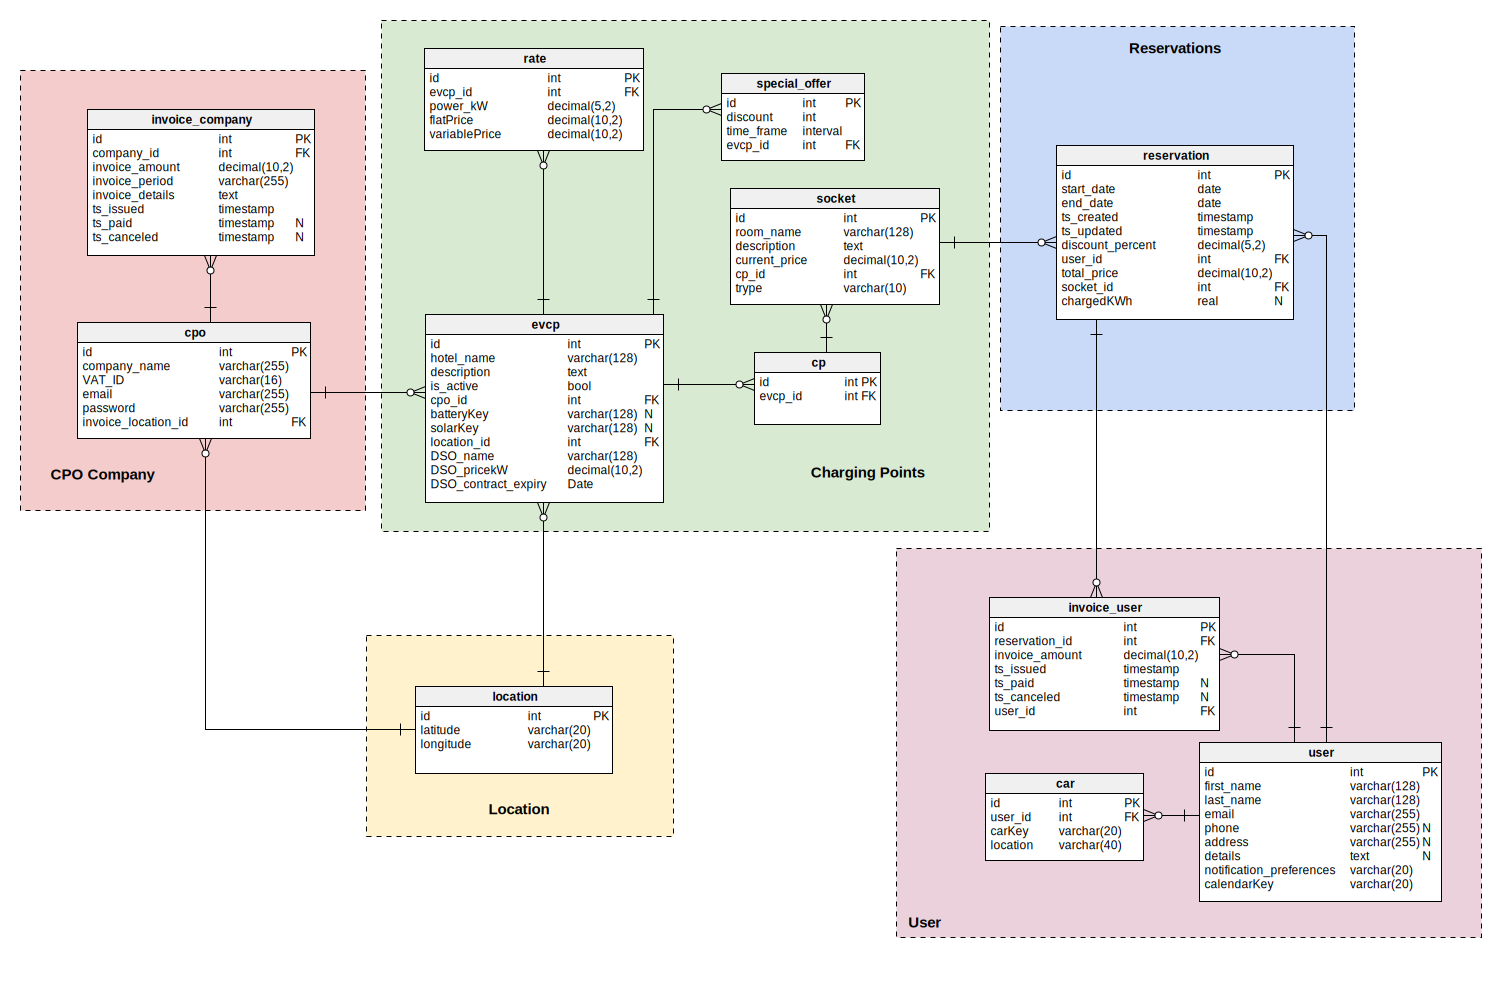
\includegraphics[scale=0.42]{src/ERDiagram/er_diagram.pdf}
\end{figure}
\pagebreak
\subsection{Deployment view}

Our system consists of two parts: a static web server and an application server. The static web server will be the entry point for clients to access the SPA, while the application server will provide the necessary APIs for the SPA to work. We have chosen to use two different solutions for these components. The static web server will be hosted on a CDN (Content Delivery Network) to ensure fast response times through its edge location caches and reverse proxies. The application server, which includes both a business logic layer and a data tier, will be hosted on a cloud provider.
This offers several advantages compared to traditional in-house hosting, such as:
\begin{itemize}
    \item Scalability and Flexibility - the ability to add or remove resources such as virtual machines, performance cores, or memory as needed, and the use of load balancing services, allows the application server to adapt to changes in traffic or workload.
    \item Security - services like live monitoring and firewalls help to protect the application server against data breaches, cyberattacks, and other security threats.
    \item Cost-efficiency - the pay-as-you-go model of a cloud provider allows to only pay for the resources that are actually used, which can help to lower the overall costs.
\end{itemize}
These features make a cloud provider an ideal choice for hosting large, high-traffic applications. The chosen cloud provider will need to offer all of these features in order to meet our needs.

\begin{figure}[H]
    \centering
    \includegraphics[scale=0.55]{src/deploymentDiagram/deployment_diagram.pdf}
    \caption{EV Driver Registration process}
\end{figure}

The deployment diagram offers a more detailed view over the hardware and software resources of the application:
\begin{itemize}
    \item PC or Mobile Device is any device having a modern browser capable of running the JavaScript based web app.
    \item The SPA will be hosted by a CDN, which will allow it to be downloaded without affecting the performance of the main application server. The SPA is static and all of its code is run on the client's machine, so there is no need for any logic to be implemented on the CDN side.
    \item The Cloud Services will host all the business and data logic for the system. It contains:
          \begin{itemize}
              \item \textbf{Firewall} services are used to filter incoming connections to the business and data layers of a system. They provide an additional layer of security by blocking or allowing traffic based on predetermined rules. This helps to protect the system from unauthorized access or malicious attacks.
              \item \textbf{Load balancer} to distribute incoming traffic across multiple instances of an application in order to optimize resource utilization, improve performance, and ensure high availability. The load balancer helps to ensure that the application can handle a large volume of requests without becoming overloaded or experiencing downtime. It also helps to provide a more stable and reliable experience for users by redirecting traffic to the least busy application instance.
              \item Multiple copies of the \textbf{application}. The various instances can run in parallel and independently to meet the demand for the application. These instances can be created or deleted as needed. Running multiple instances allows the application to handle a high volume of requests without experiencing performance issues, and provides fault tolerance by allowing traffic to be redirected to a different instance if one instance becomes unavailable.
              \item \textbf{Data Instance} which is a data optimized virtual machine containing the DBMS and the database.
          \end{itemize}
\end{itemize}



\pagebreak
\subsection{Runtime view}
The runtime views describe the interactions between actors, subsystems and interfaces of the system showing the specific method called.
The views are divided between eMSP and CPMS.

\subsubsection{Token Validation}
Users can only search and view details of a CP without first being authenticated and authorized. All other actions that a user (both drivers and CPOs) can perform are dependent on the validation of a token. The token is passed in the API request and the process of verifying it is shown in the sequence diagram below.
\begin{figure}[H]
    \centering
    \includegraphics[scale=0.75]{src/runtimeView/auth.pdf}
    \caption{User token validation}
\end{figure}

\subsubsection{eMSP}
\begin{itemize}
    \item \textbf{EV Driver Registration} : The following diagram represents the workflow that an EV Driver has to follow to register into eMall.\\
          \\When the unregistered user enters the input data the System will check whether the data input is valid. If the input is valid,
          the request is forwarded to the Account Manager that proceeds to evaluate if there is another user registered with
          the same phone number. If the user has inserted a phone number not already registered, then the user is created and an sms verification
          code is sent to the user through the SMS Service. After receiving the correct verification code the user is notified that the
          registration is completed.
          \begin{figure}[H]
              \centering
              \includegraphics[scale=0.55]{src/runtimeView/eMSP_Registration.pdf}
              \caption{EV Driver Registration process}
          \end{figure}
          \pagebreak
    \item \textbf{EV Driver Log in} : The following diagram represents the workflow that the EV Driver has to follow to log in.\\
          \\After submitting the login inputs, the Account Manager verifies the credentials by interacting with the Query Manager. If
          the input is correct authenticates the user through a token and redirects the EV Driver to the Map Homepage.
          \begin{figure}[H]
              \centering
              \includegraphics[scale=0.60]{src/runtimeView/eMSP_Login.pdf}
              \caption{EV Driver Logs in the system}
          \end{figure}
    \item \textbf{EV Driver Search an EVCP} : The following diagram represents the workflow that the EV Driver has to follow to search for CPs in the map.\\
          \\By filtering the results by location, connector and/or date sends a request for an update of the page. The CP Search
          interacts with the Query Manager to get the filtered CPs and responds with the list.
          \begin{figure}[H]
              \centering
              \includegraphics[scale=0.60]{src/runtimeView/eMSP_Search.pdf}
              \caption{EV Driver searches on the map}
          \end{figure}
          \pagebreak
    \item \textbf{EV Driver books a charge} : The following diagram represents the workflow when the EV Driver books a charge.\\
          \\After the submission of the reservation parameters by the user, the Reservation Manager interacts with the eMSPtoCPMSConnector to
          contact the specific CPMS to book the charge. The reservations parameters are received by the specific CPMStoeMSPConnector that
          forwards the payload to the Booking Manager that contacts the Query Manager to verify that the reservations parameters aren't in
          conflict with others reservations. If the reservation is valid then is added to the database through the Query Manager and the Reservation
          Manager of the eMSP is notified of the validity of the reservation. The Reservation Manager contacts the Payment Gateway to pre-authorize the
          payment with the credit card that has been already added and selected by the EV Driver.
          \begin{figure}[H]
              \centering
              \hspace*{-2cm}
              \includegraphics[scale=0.48]{src/runtimeView/eMSP_Book.pdf}
              \caption{EV Driver books a charge}
          \end{figure}
          \pagebreak
    \item \textbf{EV Driver starts a charge} : The following diagram represents the workflow when the EV Driver starts a charge.\\
          \\The submission of the request contains the reservation identifier of the charge that has to be started and the car details.
          The Reservation manager interacts with the eMSPtoCPMSConnector to contact the specific CPMS. Through the CPMStoeMSPConnector the
          Booking Manager receives the request to start a charge. Verifies through the Query Manager that the request corresponds to a reservation
          that can be started. If so, the Booking Manager contacts the Charging Points Manager to activate the socket of the CP specified in the reservation.
          The Charging Points Manager contacts the CP through the OCPP Compliant CP interface and starts the charge.
          \begin{figure}[H]
              \centering
              \hspace*{-2cm}
              \includegraphics[scale=0.50]{src/runtimeView/eMSP_StartACharge.pdf}
              \caption{EV Driver starts a charge}
          \end{figure}
    \item \textbf{EV Driver sees reservations} : The following diagram represents the workflow when the EV Driver wants to see the his/her reservations.\\
          \\ The Reservation Manager is contacted and requires the Query Manager to find all the reservations associated with the EV Driver.
          \begin{figure}[H]
              \centering
              \includegraphics[scale=0.70]{src/runtimeView/eMSP_Reservations.pdf}
              \caption{EV Driver sees the reservations}
          \end{figure}
          \pagebreak
    \item \textbf{EV Driver adds a credit card} : The following diagram represents the workflow when the EV Driver adds a credit card.\\
          \\
          \begin{figure}[H]
              \centering
              \includegraphics[scale=0.85]{src/runtimeView/eMSP_AddCC.pdf}
              \caption{EV Driver adds a credit card information}
          \end{figure}
    \item \textbf{EV Driver adds a car} : The following diagram represents the workflow when the EV Driver adds a car.\\
          \\
          \begin{figure}[H]
              \centering
              \includegraphics[scale=0.65]{src/runtimeView/eMSP_AddACar.pdf}
              \caption{EV Driver adds a car}
          \end{figure}
          \pagebreak
    \item \textbf{Suggestion} : The following diagram represents the workflow when a Suggestion is sent to the EV Driver.\\
          \\After the discharge of the car, the interface EV Service sends "lowBatteryEvent".
          The Suggestion Manager receives carID such that can obtain through the Query Manager, from the DB, the corresponding userID.
          The Suggestion Manager, thanks to the attribute calendar "key" of the user, interacts with the Calendar API and receives "FreeSpots" (those
          time intervals in the user Calendar that are free).
          The Suggestion Manager contacts the Query Manager with "getTopKSuggestions" through which obtains the top K suggestions according
          to the ranking algorithm implemented by the system.
          The Suggestion Manager contacts Notification Manager through which contacts the Query Manager to find the notification preferences.
          If the notification preferences of the user are such that he accepts suggestion, the Notification Manager pushes a notification through the Push Notification Service.
          \\
          \begin{figure}[H]
              \centering
              \hspace*{-2cm}
              \includegraphics[scale=0.48]{src/runtimeView/eMSP_Suggestion.pdf}
              \caption{Suggestion}
          \end{figure}
          \pagebreak
    \item \textbf{Current Charge Info}: The following diagram represents the workflow when the EV Driver wants to see details of the current charge.\\
          \\The Reservation Manager receives a request from a driver for reservation details and uses the connector to cpms to contact the specific CPMS of the CPO that owns the charging point where the reservation is taking place. The CPMS then sends a request for meter values to the charging point via the OCPP protocol and receives a response with the requested information. This information is then passed back through the system and displayed to the driver through the web app.
          \\\begin{figure}[H]
              \centering
              \hspace*{-2cm}
              \includegraphics[scale=0.45]{src/runtimeView/eMSP_currentChargeInfo.pdf}
              \caption{EV sees the current charge information}
          \end{figure}
\end{itemize}

\subsubsection{CPMS}
\begin{itemize}
    \item \textbf{CPO sees the reservations} : The following diagram represents the workflow when the CPO wants to see the his/her reservations.\\
          \begin{figure}[H]
              \centering
              \includegraphics[scale=0.75]{src/runtimeView/CPMS_Reservations.pdf}
              \caption{CPO sees the reservations}
          \end{figure}
          \pagebreak
    \item \textbf{CPO adds a Charging Point} : The following diagram represents the workflow when the CPO adds a charging point.\\
          \\ The request contains the information about the CP unique identifier, the EVCP in which the CP is going to be added, and the rate associated with.
          The Charging Points Manager interacts with the Query Manager to add the information. When the user, through the CP manufacturer's portal connects the
          CP to the CPMS, then the CP is connected and is able to receive OCPP messages from the CPMS of the CPO.
          \begin{figure}[H]
              \centering
              \includegraphics[scale=0.75]{src/runtimeView/CPMS_AddCP.pdf}
              \caption{CPO adds a Charging Point}
          \end{figure}
    \item \textbf{CPO adds a rate} : The following diagram represents the workflow when the CPO adds a rate.\\
          \\
          \begin{figure}[H]
              \centering
              \includegraphics[scale=0.80]{src/runtimeView/CPMS_addRate.pdf}
              \caption{CPO adds a rate}
          \end{figure}
          \pagebreak
    \item \textbf{CPO sees the energy storage system capacity} : The following diagram represents the workflow when the CPO wants to see the energy storage system capacity.\\
          \\ The request contains the specific EVCP identifier of where the energy storage system is located. The Energy Manager requires to the database the unique key to access
          to the API of the Energy Storage. Then asks the Energy Storage API the information about the status.
          \begin{figure}[H]
              \centering
              \includegraphics[scale=0.75]{src/runtimeView/CPMS_batteryCapacity.pdf}
              \caption{CPO sees the energy storage system capacity}
          \end{figure}
    \item \textbf{CPO sees the status of its Charging Points} : The following diagram represents the workflow when the CPO wants to see the charging points status of an evcp.\\
          \\ The request contains the specific EVCP identifier of where the CPs are located. The Charging Points manager asks the Query Manager for a list of CPs of the specific EVCP
          and the contacts each one of the CP from the list with the OCPP Compliant CP interface.
          \begin{figure}[H]
              \centering
              \includegraphics[scale=0.70]{src/runtimeView/CPMS_CPsStatus.pdf}
              \caption{CPO sees the status of its Charging Points}
          \end{figure}
          \pagebreak
    \item \textbf{CPO adds a special offer} : The following diagram represents the workflow when the CPO adds a special offer.\\
          \\
          \begin{figure}[H]
              \centering
              \includegraphics[scale=0.75]{src/runtimeView/CPMS_specialOffer.pdf}
              \caption{CPO adds a special offer}
          \end{figure}
    \item \textbf{Choose energy Mix} : The following diagram represents the workflow when the CPO chooses the energy mix.\\
          \\ The CPO changes energy mix interacting with the Energy Manager. The Energy Manager interacts with the Query Manager obtaining the battery and solar keys.
          Then, the Energy Manager with this information and the mix attribute contacts the Energy Storage API and obtains the new mix.
          \begin{figure}[H]
              \centering
              \includegraphics[scale=0.65]{src/runtimeView/CPMS_energyMix.pdf}
              \caption{CPO chooses energy Mix}
          \end{figure}
          \pagebreak
    \item \textbf{Choose DSO} : The following diagram represents the workflow when the CPO chooses DSO.\\
          \\ The CPO chooses DSO interacting with the Energy Manager. The Energy Manager interacts with the Query Manager obtaining the Commitment Date of the actual contract.
          If the Commitment date is not reached yet, the Energy Manager responds that the request is not valid.
          Otherwise, the Energy Manager interacts with the Energy Storage API obtaining a contract. Then the Energy Manager sends an ACK to the CPO and interacts with the
          Query Manager to store the new contract.
          \begin{figure}[H]
              \centering
              \includegraphics[scale=0.60]{src/runtimeView/CPMS_chooseDSO.pdf}
              \caption{CPO chooses a DSO to acquire energy from}
          \end{figure}
\end{itemize}
\pagebreak
\subsection{Component interfaces}
In this section, we use a class diagram to illustrate the component interfaces. The methods are presented as clearly as possible, and we expect their functionality to be easily understandable.
\begin{figure}[H]
    \centering
    \hspace*{-2.5cm}
    \includegraphics[scale=0.6]{src/componentInterfaces/overview_interface.pdf}
    \caption{Class Diagram with interfaces of the eMall System}
\end{figure}
\begin{figure}[hp]
    \centering
    \hspace*{-2.5cm}
    \includegraphics[scale=0.55]{src/componentInterfaces/emsp_interface.pdf}
    \caption{Class Diagram with interfaces of the eMSP System}
\end{figure}
\begin{figure}[H]
    \centering
    \hspace*{-2.5cm}
    \includegraphics[scale=0.5]{src/componentInterfaces/cpms_interface.pdf}
    \caption{Class Diagram with interfaces of the CPMS System}
\end{figure}

\subsubsection{API endpoints}
In this section the API endpoints are presented. The focus is on the method used, on the parameters required and on the response.

\section*{Endpoint: api/cpo/user/signup}
\subsection*{Method: POST}
\subsubsection*{Request Body}
\begin{itemize}
    \item companyName: String
    \item email: String
    \item password: String
\end{itemize}
\subsubsection*{Response}
\begin{itemize}
    \item 200
          \begin{itemize}
              \item message: String ("A verification code is sent via mail")
              \item id: number
          \end{itemize}
    \item 400
          \begin{itemize}
              \item error: String ("eMail not valid", "Password must contain at least 8 character (at least one uppercase), at least 1 special symbol and at least 1 number")
          \end{itemize}
    \item 409
          \begin{itemize}
              \item error: String ("An account with the same email already exist, retry")
          \end{itemize}
\end{itemize}

\section*{Endpoint: api/cpo/user/code}
\subsection*{Method: POST}
\subsubsection*{Request Body}
\begin{itemize}
    \item cpoID: number
    \item code: String (6-digit number)
\end{itemize}
\subsubsection*{Response}
\begin{itemize}
    \item 200
          \begin{itemize}
              \item message: String ("Code inserted is valid, user verified")
          \end{itemize}
    \item 400
          \begin{itemize}
              \item error: String ("Code must be a six-digit number", "Wrong code, retry")
              \item id: number (if error is "Wrong code, retry")
          \end{itemize}
    \item 409
          \begin{itemize}
              \item error: String ("Intrusion")
          \end{itemize}
    \item 410
          \begin{itemize}
              \item error: String ("Too late, the code is expired. Register a new account.")
          \end{itemize}
\end{itemize}

\section*{Endpoint: api/cpo/user/login}
\subsection*{Method: POST}
\subsubsection*{Request Body}
\begin{itemize}
    \item email: String
    \item password: String
\end{itemize}
\subsubsection*{Response}
\begin{itemize}
    \item 200
          \begin{itemize}
              \item message: String ("Cookie Token has been set")
          \end{itemize}
    \item 400
          \begin{itemize}
              \item error: String ("eMail not valid", "Password must contain at least 8 character (at least one uppercase), at least 1 special symbol and at least 1 number")
          \end{itemize}
    \item 401
          \begin{itemize}
              \item error: String ("Email or Password are wrong")
          \end{itemize}
    \item 410
          \begin{itemize}
              \item error: String ("User not verified. Register a new account.")
          \end{itemize}
\end{itemize}

\section*{Endpoint: api/cpo/book/:evcpID}
\subsection*{Method: GET}
\subsubsection*{URL Parameters}
\begin{itemize}
    \item evcpID: number
\end{itemize}
\subsubsection*{Response}
\begin{itemize}
    \item 200
          \begin{itemize}
              \item reservations: Array of Objects
                    \begin{itemize}
                        \item id: number
                        \item evcpID: number
                        \item driverID: number
                        \item start: String (date)
                        \item end: String (date)
                    \end{itemize}
          \end{itemize}
    \item 401
          \begin{itemize}
              \item error: String ("Unauthorized")
          \end{itemize}
\end{itemize}

\section*{Endpoint: api/cpo/book/}
\subsection*{Method: GET}
\subsubsection*{Response}
\begin{itemize}
    \item 200
          \begin{itemize}
              \item aggregated: Array of Objects
                    \begin{itemize}
                        \item evcpID: number
                        \item date: String (date)
                        \item profit: number
                    \end{itemize}
          \end{itemize}
    \item 401
          \begin{itemize}
              \item error: String ("Unauthorized")
          \end{itemize}
\end{itemize}

\section*{Endpoint: api/cpo/cp/}
\subsection*{Method: GET}
\subsubsection*{Response}
\begin{itemize}
    \item 200
          \begin{itemize}
              \item EVCPs: Array of Objects
          \end{itemize}
    \item 401
          \begin{itemize}
              \item error: String ("Unauthorized")
          \end{itemize}
\end{itemize}

\section*{Endpoint: api/cpo/cp/:evcpID}
\subsection*{Method: GET}
\subsubsection*{URL Parameters}
\begin{itemize}
    \item evcpID: number
\end{itemize}
\subsubsection*{Response}
\begin{itemize}
    \item 200
          \begin{itemize}
              \item evcpDetails: Array of Objects
          \end{itemize}
    \item 401
          \begin{itemize}
              \item error: String ("Unauthorized")
          \end{itemize}
\end{itemize}

\section*{Endpoint: api/cpo/cp/}
\subsection*{Method: POST}
\subsubsection*{Request Body}
\begin{itemize}
    \item name: String
    \item latitude: number
    \item longitude: number
    \item address: String
\end{itemize}
\subsubsection*{Response}
\begin{itemize}
    \item 200
          \begin{itemize}
              \item message: String ("EVCP added")
          \end{itemize}
    \item 401
          \begin{itemize}
              \item error: String ("Unauthorized")
          \end{itemize}
    \item 409
          \begin{itemize}
              \item error: String ("An EVCP in the same spot already exists")
          \end{itemize}
\end{itemize}

\section*{Endpoint: api/cpo/cp/:evcpID}
\subsection*{Method: POST}
\subsubsection*{URL Parameters}
\begin{itemize}
    \item evcpID: number
\end{itemize}
\subsubsection*{Response}
\begin{itemize}
    \item 200
          \begin{itemize}
              \item message: String ("CP added")
          \end{itemize}
    \item 400
          \begin{itemize}
              \item error: String ("EVCP not found")
          \end{itemize}
    \item 401
          \begin{itemize}
              \item error: String ("Unauthorized")
          \end{itemize}
\end{itemize}

\section*{Endpoint: api/cpo/cp/:cpID}
\subsection*{Method: POST}
\subsubsection*{URL Parameters}
\begin{itemize}
    \item cpID: number
\end{itemize}
\subsubsection*{Request Body}
\begin{itemize}
    \item power: number
    \item type: String
\end{itemize}
\subsubsection*{Response}
\begin{itemize}
    \item 200
          \begin{itemize}
              \item message: String ("Socket added")
          \end{itemize}
    \item 400
          \begin{itemize}
              \item error: String ("CP not found")
          \end{itemize}
    \item 401
          \begin{itemize}
              \item error: String ("Unauthorized")
          \end{itemize}
\end{itemize}

\section*{Endpoint: api/cpo/energy/:evcpID}
\subsection*{Method: GET}
\subsubsection*{URL Parameters}
\begin{itemize}
    \item evcpID: number
\end{itemize}
\subsubsection*{Response}
\begin{itemize}
    \item 200
          \begin{itemize}
              \item dso: Object (Name, contract, price)
          \end{itemize}
    \item 401
          \begin{itemize}
              \item error: String ("Unauthorized")
          \end{itemize}
\end{itemize}

\section*{Endpoint: api/cpo/energy/dso/:evcpID}
\subsection*{Method: GET}
\subsubsection*{URL Parameters}
\begin{itemize}
    \item evcpID: number
\end{itemize}
\subsubsection*{Response}
\begin{itemize}
    \item 200
          \begin{itemize}
              \item availableDSOs: Array of Objects
          \end{itemize}
    \item 401
          \begin{itemize}
              \item error: String ("Unauthorized")
          \end{itemize}
\end{itemize}

\section*{Endpoint: api/cpo/energy/dso/:evcpID}
\subsection*{Method: POST}
\subsubsection*{URL Parameters}
\begin{itemize}
    \item evcpID: number
\end{itemize}
\subsubsection*{Request Body}
\begin{itemize}
    \item dsoID: number
\end{itemize}
\subsubsection*{Response}
\begin{itemize}
    \item 200
          \begin{itemize}
              \item message: String ("DSO updated")
          \end{itemize}
    \item 400
          \begin{itemize}
              \item error: String ("DSO not available")
          \end{itemize}
    \item 401
          \begin{itemize}
              \item error: String ("Unauthorized")
          \end{itemize}
\end{itemize}

\section*{Endpoint: api/cpo/rate/:evcpID}
\subsection*{Method: POST}
\subsubsection*{URL Parameters}
\begin{itemize}
    \item evcpID: number
\end{itemize}
\subsubsection*{Request Body}
\begin{itemize}
    \item typeName: String
    \item flatPrice: number
    \item variablePrice: number
\end{itemize}
\subsubsection*{Response}
\begin{itemize}
    \item 200
          \begin{itemize}
              \item message: String ("Rate added")
          \end{itemize}
    \item 400
          \begin{itemize}
              \item error: String ("EVCP not found")
          \end{itemize}
    \item 401
          \begin{itemize}
              \item error: String ("Unauthorized")
          \end{itemize}
\end{itemize}

\section*{Endpoint: api/cpo/rate/:evcpID}
\subsection*{Method: GET}
\subsubsection*{URL Parameters}
\begin{itemize}
    \item evcpID: number
\end{itemize}
\subsubsection*{Response}
\begin{itemize}
    \item 200
          \begin{itemize}
              \item rates: Array of Objects
          \end{itemize}
    \item 401
          \begin{itemize}
              \item error: String ("Unauthorized")
          \end{itemize}
\end{itemize}

\section*{Endpoint: api/driver/user/signup}
\subsection*{Method: POST}
\subsubsection*{Request Body}
\begin{itemize}
    \item firstName: String
    \item lastName: String
    \item phoneNumber: String
    \item password: String
\end{itemize}
\subsubsection*{Response}
\begin{itemize}
    \item 200
          \begin{itemize}
              \item message: String ("A verification code is sent via SMS")
              \item id: number
          \end{itemize}
    \item 400
          \begin{itemize}
              \item error: String ("Phone number not valid","Password must contain at least 8 character (at least one uppercase), at least 1 special symbol and at least 1 number")
          \end{itemize}
    \item 409
          \begin{itemize}
              \item error: String ("An account with the same phone number already exist, retry")
          \end{itemize}
\end{itemize}

\section*{Endpoint: api/driver/user/code}
\subsection*{Method: POST}
\subsubsection*{Request Body}
\begin{itemize}
    \item driverID: number
    \item code: number (6-digit code)
\end{itemize}
\subsubsection*{Response}
\begin{itemize}
    \item 200
          \begin{itemize}
              \item message: String ("A verification code is sent via SMS")
              \item id: number
          \end{itemize}
    \item 400
          \begin{itemize}
              \item error: String ("Code must be a six-digit number","Wrong code, retry")
              \item id: number (if error is "Wrong code, retry")
          \end{itemize}
    \item 410
          \begin{itemize}
              \item error: String ("Too late, the code is expired. Register a new account")
          \end{itemize}
\end{itemize}

\section*{Endpoint: api/driver/user/login}
\subsection*{Method: POST}
\subsubsection*{Request Body}
\begin{itemize}
    \item phoneNumber: String
    \item password: String
\end{itemize}
\subsubsection*{Response}
\begin{itemize}
    \item 200
          \begin{itemize}
              \item message: String ("Cookie Token is set")
          \end{itemize}
    \item 400
          \begin{itemize}
              \item error: String ("Phone number not valid")
          \end{itemize}à
    \item 401
          \begin{itemize}
              \item error: String ("Phone number or Password are wrong")
          \end{itemize}
    \item 410
          \begin{itemize}
              \item error: String ("User not verified. Register a new account")
          \end{itemize}
\end{itemize}

\section*{Endpoint: api/driver/user/notification}
\subsection*{Method: PATCH}
\subsubsection*{Request Body}
\begin{itemize}
    \item notificationToken: String
\end{itemize}
\subsubsection*{Response}
\begin{itemize}
    \item 200
          \begin{itemize}
              \item message: String ("Notification Token Set Correctly")
          \end{itemize}
    \item 401
          \begin{itemize}
              \item error: String ("Unauthorized")
          \end{itemize}
\end{itemize}

\section*{Endpoint: api/driver/search}
\subsection*{Method: GET}
\subsubsection*{URL Query Parameters}
\begin{itemize}
    \item latitude: number
    \item longitude: number
    \item filters: Array of Objects
\end{itemize}
\subsubsection*{Response}
\begin{itemize}
    \item 200
          \begin{itemize}
              \item EVCPs: Array of Objects
          \end{itemize}
\end{itemize}

\section*{Endpoint: api/driver/search/:evcpID}
\subsection*{Method: GET}
\subsubsection*{URL Parameters}
\begin{itemize}
    \item evcpID: number
\end{itemize}
\subsubsection*{Response}
\begin{itemize}
    \item 200
          \begin{itemize}
              \item evcpDetails: Array of Objects
          \end{itemize}
\end{itemize}

\section*{Endpoint: api/driver/reserve}
\subsection*{Method: GET}
\subsubsection*{Response}
\begin{itemize}
    \item 200
          \begin{itemize}
              \item listOfReservations: Array of Objects
          \end{itemize}
    \item 401
          \begin{itemize}
              \item error: String ("Unauthorized")
          \end{itemize}
\end{itemize}

\section*{Endpoint: api/driver/reserve/slot/:evcpID}
\subsection*{Method: GET}
\subsubsection*{URL Parameters}
\begin{itemize}
    \item evcpID: number
\end{itemize}
\subsubsection*{URL Query Parameters}
\begin{itemize}
    \item socketType: String
    \item power: number
    \item date: String
\end{itemize}
\subsubsection*{Response}
\begin{itemize}
    \item 200
          \begin{itemize}
              \item availableSlots: Array of Objects
          \end{itemize}
    \item 401
          \begin{itemize}
              \item error: String ("Unauthorized")
          \end{itemize}
\end{itemize}

\section*{Endpoint: api/driver/reserve/duration/:evcpID}
\subsection*{Method: GET}
\subsubsection*{URL Parameters}
\begin{itemize}
    \item evcpID: number
\end{itemize}
\subsubsection*{URL Query Parameters}
\begin{itemize}
    \item socketType: String
    \item power: number
    \item date: String
\end{itemize}
\subsubsection*{Response}
\begin{itemize}
    \item 200
          \begin{itemize}
              \item maxDurations: Array of Objects
          \end{itemize}
    \item 401
          \begin{itemize}
              \item error: String ("Unauthorized")
          \end{itemize}
\end{itemize}

\section*{Endpoint: api/driver/reserve/:evcpID}
\subsection*{Method: POST}
\subsubsection*{URL Parameters}
\begin{itemize}
    \item evcpID: number
\end{itemize}
\subsubsection*{Request Body}
\begin{itemize}
    \item socketType: String
    \item power: number
    \item timeFrom: String (date)
    \item timeTo: String (date)
\end{itemize}
\subsubsection*{Response}
\begin{itemize}
    \item 200
          \begin{itemize}
              \item message: String ("The reservation has been accepted")
          \end{itemize}
    \item 401
          \begin{itemize}
              \item error: String ("Unauthorized")
          \end{itemize}
    \item 409
          \begin{itemize}
              \item error: String ("Conflict")
          \end{itemize}
\end{itemize}

\section*{Endpoint: api/driver/reserve/start/:reservationID}
\subsection*{Method: POST}
\subsubsection*{URL Parameters}
\begin{itemize}
    \item reservationID: number
\end{itemize}
\subsubsection*{Response}
\begin{itemize}
    \item 200
          \begin{itemize}
              \item message: String ("The charging has been started")
          \end{itemize}
    \item 401
          \begin{itemize}
              \item error: String ("Unauthorized")
          \end{itemize}
    \item 404
          \begin{itemize}
              \item error: String ("Charging not started, error")
          \end{itemize}
\end{itemize}

\section*{Endpoint: api/driver/car/:carID}
\subsection*{Method: GET}
\subsubsection*{URL Parameters}
\begin{itemize}
    \item carID: number
\end{itemize}
\subsubsection*{Response}
\begin{itemize}
    \item 200
          \begin{itemize}
              \item chargeDetails: Array of Objects
          \end{itemize}
    \item 401
          \begin{itemize}
              \item error: String ("Unauthorized")
          \end{itemize}
\end{itemize}

\subsection{Architectural Styles and patterns}
\begin{itemize}
    \item \textbf{Three layers and Four Tier}\\
          We decided to use a three-layer, four-tier architecture for our software system because it offers several benefits. First, it allows us to divide the system into distinct layers (presentation, business logic, data access) and tiers (client, static web server, application server, DBMS), which makes the system more modular and easier to modify or maintain. It also enables us to reuse code and components across different layers and tiers. Additionally, the separation of the layers and tiers allows us to scale the system more easily by distributing the workload across multiple servers. Finally, the architecture enables the use of load balancing and caching techniques to improve performance.
    \item \textbf{RESTful APIs}\\
          We chose to use a REST API as the backend for the frontend application because it offers several benefits. The API is based on standard web technologies, making it easy to consume and integrate with other systems. It is stateless, which simplifies the development. Additionally, the REST API is scalable, which can improve the overall performance of the system.
    \item \textbf{Adapter Pattern}\\
          The Query Manager component acts as an adapter between the business logic and the DBMS services. It provides a simplified interface for accessing the DBMS, while hiding the underlying complexity and exposing only a limited set of high-level functions.
\end{itemize}
\subsection{Other design decisions}
\subsubsection{PWA}
The decision to build the web application as a PWA for drivers was made in order to improve the offline functionality, performance, and app-like experience of the application, as well as making it easier to install. This design choice enables the web application to work offline or with a low-quality network connection, using service workers to store assets and data locally. The PWA also improves performance by reducing the need for network requests and loading faster due to the use of service workers. Finally, the PWA can be easily installed on the user's device, similar to a native mobile app, making it convenient for drivers to access the application.
\subsubsection{Scale-out}
The decision to implement a scale out design in the software was taken to enhance its ability to scale, its availability, and its performance. This design approach enables the system to expand its capacity to cope with increased demand by adding more resources, such as servers or machines, as needed. This can be more cost-effective than upgrading individual components and avoids the need for downtime. The scale out design also improves the system's reliability by providing redundant resources that can take over if any component fails. In addition, the design allows for flexibility, as resources can be added or removed as required. Lastly, the scale out design improves the system's performance by allowing workloads to be processed in parallel rather than sequentially.

\subsubsection{Relational Database}
We selected a relational database for our system design because it is effective at storing structured data, enforcing data integrity, and providing fast query performance. It can also scale to handle large amounts of data and support many concurrent users. The database allows us to store and retrieve information efficiently, while also ensuring that the data is accurate and consistent.
\subsubsection{The separation of eMSP and CPMSs}
The decision to design eMSP and CPMSs as independent entities is driven by the need to maintain a consistent interface between them that follows a standard protocol. While this may initially lead to the duplication of some common components, it is necessary because the systems have distinct roles. As the operating environment is subject to change, it is possible that future standard protocols will require eMSP and CPMS to follow a single protocol for searching and booking CPs. By designing them as independent entities, it will be easier to incorporate any new protocol and enable eMSP to access CPMSs even from CPOs not directly subscribed to the system.
\section{User Interface Design}
In RASD we already did mockups so here we put UX flowcharts.
Overview of UIs, possibly mockups, may refine what's in the RASD (if present)

\begin{figure}[H]
    \centering
    \includegraphics[scale=0.41]{src/UIDesign/User.pdf}
    \caption{EVdriver}
\end{figure} \vspace{1cm}

\begin{figure}[H]
    \centering
    \includegraphics[scale=0.41]{src/UIDesign/Cpo.pdf}
    \caption{Charging Point Operator}
\end{figure} \vspace{1cm}
\section{Requirements traceability}
Explain how the requirements you have defined in the RASD map to the design elements that you have defined in this document.
\section{Implementation, integration and testing plan}
Identify here the order in which you plan
to implement the subcomponents of your system and the order in which you plan to integrate
such subcomponents and test the integration
\section{Effort Spent}
\subsection*{Pair working}
\begin{table}[H]
    \begin{tabular}{lr}
        \toprule
        \textbf{DD Structure analysis, overview architecture brainstorming} & \textbf{4h}   \\
        \textbf{Component Diagram}                                          & \textbf{5h}   \\
        \textbf{Runtime View}                                               & \textbf{8h}   \\
        \textbf{Database Entity Relationship Diagram}                       & \textbf{2h}   \\
        \textbf{Final Review}                                               & \textbf{2.5h} \\
        \bottomrule
    \end{tabular}
\end{table}

\subsection*{Giovanni}
\begin{table}[H]
    \begin{tabular}{lr}
        \toprule
        \textbf{Introduction section}                          & \textbf{1h}   \\
        \textbf{Deployment View}                               & \textbf{1.5h} \\
        \textbf{Review: ER Diagram}                            & \textbf{1.5h} \\
        \textbf{NFR Traceability}                              & \textbf{1h}   \\
        \textbf{Component Interfaces: diagram and description} & \textbf{2.5h}   \\
        \textbf{Design Choices description}                    & \textbf{0.5h} \\
        \bottomrule
    \end{tabular}
\end{table}

\subsection*{Matteo}
\begin{table}[H]
    \begin{tabular}{lr}
        \toprule
        \textbf{Requirements traceability} & \textbf{5h} \\
        \textbf{Component Diagram}         & \textbf{1h} \\
        \bottomrule
    \end{tabular}
\end{table}

\subsection*{Lorenzo}
\begin{table}[H]
    \begin{tabular}{lr}
        \toprule
        \textbf{User Interface Design} & \textbf{3h} \\
        \textbf{Development process and approach} & \textbf{1.5h} \\
        \textbf{Implementation Plan} & \textbf{1h} \\
        \textbf{Integration Plan} & \textbf{4h} \\
        \textbf{System Testing} & \textbf{0.5h} \\
        \bottomrule
    \end{tabular}
\end{table}

\section{References}
\begin{itemize}
    \item Software Engineering II course slides
    \item Use Case Diagrams were made using draw.io\\ \url{https://app.diagrams.net/}
    \item All other diagrams were made using StarUML\\ \url{https://staruml.io/}
\end{itemize}

\end{document}